\section{Evaluation}

To evaluate our functional conversion scheme, we implemented the proposed algorithm in \haskell.
We compared execution time of several \ocanren relations in different directions against their functional counterparts in the \ocaml language.
Here we showcase two relational programs and their conversions.
The implementation of the functional conversion\footnote{The repository of the functional conversion project \url{https://github.com/kajigor/uKanren_transformations}} as well as the execution code\footnote{Evaluation code \url{https://github.com/kajigor/miniKanren-func}} can be found on Github.

\begin{figure}[h]
  \centering
  \begin{subfigure}[b]{0.45\textwidth}
    \begin{lstlisting}[frame=tb]
let rec eval$^o$ st$^{g \to g}$ fm$^{f \to g}$ u$^{g \to g}$ =
  ( fm$^{f \to g}$  ===    Lit u$^{g \to g}$) \/
  ( elem$^o$ z$^{f \to g}$ st$^{g \to g}$ u$^{g \to g}$ /\
    fm$^{f \to g}$ ===    Var z$^{g \to g}$ ) \/
  ( not$^o$ v$^{f \to g}$ u$^{g \to g}$ /\
    eval$^o$ st$^{g \to g}$ x$^{f \to g}$ v$^{g \to g}$ /\
    fm$^{f \to g}$ ===    Neg x$^{g \to g}$ ) \/
  ( or$^o$ v$^{f \to g}$ w$^{f \to g}$ u$^{g \to g}$ /\
    eval$^o$ st$^{g \to g}$ x$^{f \to g}$ v$^{g \to g}$ /\
    eval$^o$ st$^{g \to g}$ y$^{f \to g}$ w$^{g \to g}$ /\
    fm$^{f \to g}$ ===    Disj x$^{g \to g}$ y$^{g \to g}$) \/
  ( and$^o$ v$^{f \to g}$ w$^{f \to g}$ u$^{g \to g}$ /\
    eval$^o$ st$^{g \to g}$ x$^{f \to g}$ v$^{g \to g}$ /\
    eval$^o$ st$^{g \to g}$ y$^{f \to g}$ w$^{g \to g}$ /\
    fm$^{f \to g}$ ===    Conj x$^{g \to g}$ y$^{g \to g}$) \/
    \end{lstlisting}
   \caption{Mode inference result}
    \label{fig:prop_modded}
  \end{subfigure}
  \hfill
  \begin{subfigure}[b]{0.45\textwidth}
    \begin{lstlisting}[frame=tb]
evaloIOI x0 x2 = msum
  [ do { let {x1 = Lit x2}
       ; return x1 }
  , do { x7 <- elemoOII x0 x2
       ; let {x1 = Var x7}
       ; return x1 }
  , do { x5 <- notoOI x2
       ; x3 <- evaloIOI x0 x5
       ; let {x1 = Neg x3}
       ; return x1 }
  , do { (x5, x6) <- oroOOI x2
       ; x3 <- evaloIOI x0 x5
       ; x4 <- evaloIOI x0 x6
       ; let {x1 = Disj x3 x4}
       ; return x1 }
  , do { (x5, x6) <- andoOOI x2
       ; x3 <- evaloIOI x0 x5
       ; x4 <- evaloIOI x0 x6
       ; let {x1 = Conj x3 x4}
       ; return x1 } ]
    \end{lstlisting}
    \caption{Functional conversion}
    \label{fig:prop_hsk}
  \end{subfigure}
  \caption{Evaluator of propositional formulas}
  \label{fig:prop}
\end{figure}


\subsection{Evaluator of Propositional Formulas}

In this example, we converted a relational evaluator of propositional formulas: see figure~\ref{fig:prop}.
It evaluates a propositional formula \lstinline{fm} in the environment \lstinline{st} to get the result \lstinline{u}.
A formula is either a boolean literal, a numbered variable, a negation of another formula, a conjunction or a disjunction of two formulas.
Converting it in the direction when everything but the formula is \inm (see figure~\ref{fig:prop_modded}), allows one to synthesize formulas which can be evaluated to the given value.
The conversion of this relation does not involve any generators and is presented in figure~\ref{fig:prop_hsk}.

We run an experiment to compare execution time of the relational interpreter vs. its functional conversion.
In the experiment, we generated from $1000$ to $10000$ formulas which evaluate to true and contain up to $3$ variables with known values.
The results are presented in figure~\ref{fig:prop_time}.
The functional conversion improved execution time of the query about $2.5$ times from $724ms$ to $291ms$ for retrieving $10000$ formulas.

\begin{figure}[h]
  \centering
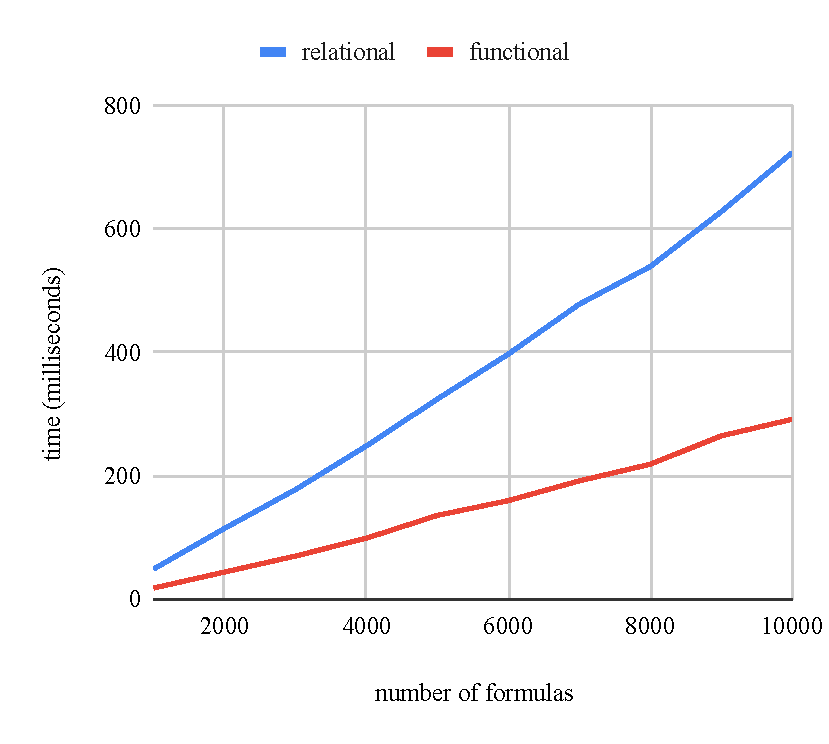
\includegraphics[width=0.49\textwidth]{fig/propIOI.pdf}
  \caption{Execution time of the evaluators of propositional formulas, \lstinline{eval [true; false; true] q true}}
  \label{fig:prop_time}
\end{figure}
 

\begin{figure}[h]
  \centering
    \begin{subfigure}[b]{0.49\textwidth}
      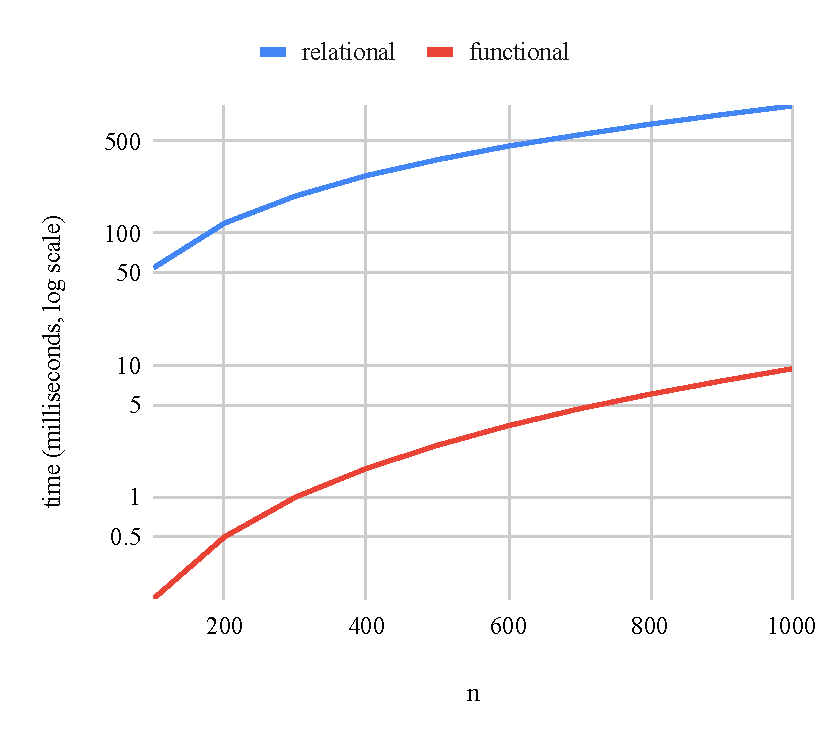
\includegraphics[width=\textwidth]{fig/muloIIO.pdf}
    \caption{Multiplication: \lstinline{mulo n 10 q}}
    \label{fig:mulo_IIO}
  \end{subfigure}
\hfill
    \begin{subfigure}[b]{0.49\textwidth}
      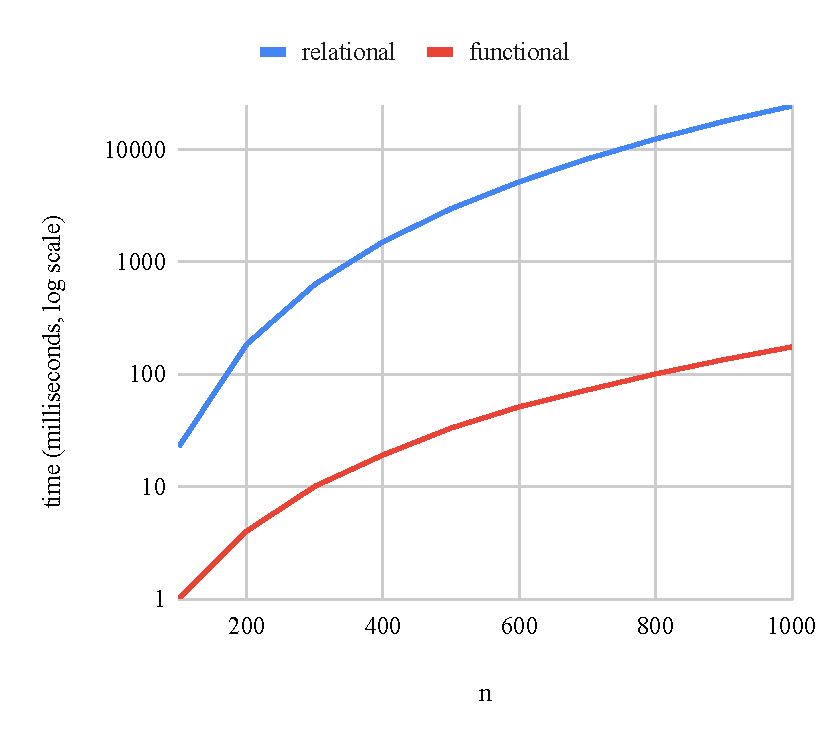
\includegraphics[width=1\textwidth]{fig/muloIOI.pdf}
    \caption{Division: \lstinline{mulo (n/10) q n}}
    \label{fig:mulo_IOI}
  \end{subfigure}

\hfill

    \begin{subfigure}[b]{0.49\textwidth}
      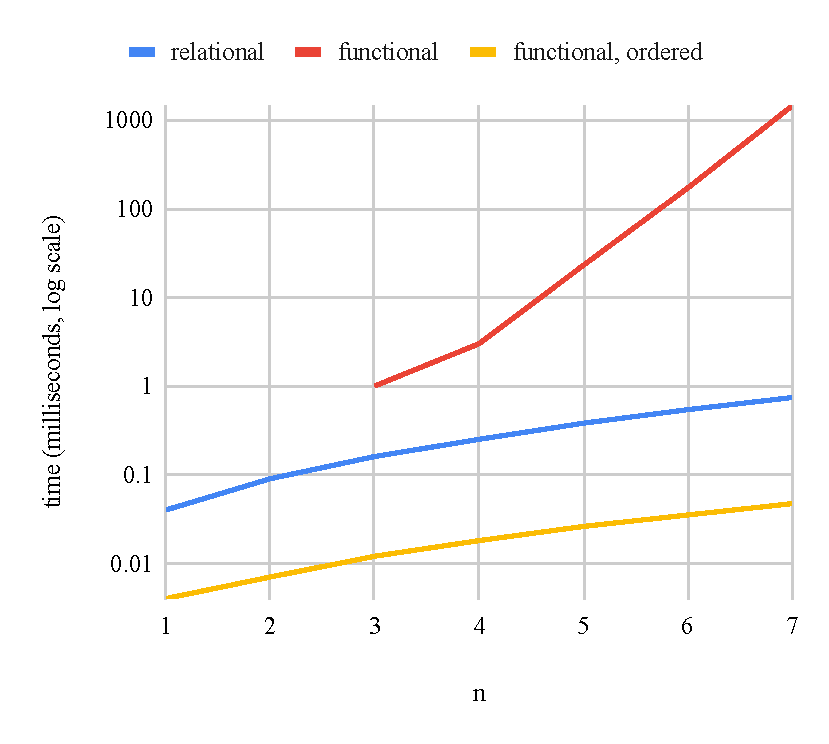
\includegraphics[width=\textwidth]{fig/muloIOO.pdf}
    \caption{Generation: \lstinline{take n (mulo 10 q r)}}
    \label{fig:mulo_IOO}
  \end{subfigure}
\hfill
  \begin{subfigure}[b]{0.45\textwidth}
    \begin{subfigure}[b]{\textwidth}
    \begin{lstlisting}[frame=tb]
let rec mul$^o$ x$^{g \rightarrow g}$ y$^{f \rightarrow g}$ z$^{f \rightarrow g}$ =
  (x$^{g \rightarrow g}$ ===    O /\ z$^{f \rightarrow g}$ ===    O) \/
  (x$^{g \rightarrow g}$ ===    S x$_1^{f \rightarrow g}$ /\
   add$^o$ y$^{f \rightarrow g}$ z$_1^{f \rightarrow g}$ z$^{f \rightarrow g}$ /\
   mul$^o$ x$_1^{g \rightarrow g}$ y$^{g \rightarrow g}$ z$_1^{g \rightarrow g}$ )
    \end{lstlisting}
    \caption{Inefficient mode}
    \label{fig:mult_modded_bad}
  \end{subfigure}
  \hfill

    \begin{subfigure}[b]{\textwidth}
    \begin{lstlisting}[frame=tb]
let rec mul$^o$ x$^{g \rightarrow g}$ y$^{f \rightarrow g}$ z$^{f \rightarrow g}$ =
  (x$^{g \rightarrow g}$ ===    O /\ z$^{f \rightarrow g}$ ===    O) \/
  (x$^{g \rightarrow g}$ ===    S x$_1^{f \rightarrow g}$) /\
   mul$^o$ x$_1^{g \rightarrow g}$ y$^{f \rightarrow g}$ z$_1^{f \rightarrow g}$ /\
   add$^o$ y$^{g \rightarrow g}$ z$_1^{g \rightarrow g}$ z$^{f \rightarrow g}$ )
    \end{lstlisting}
    \caption{Efficient mode}
    \label{fig:mult_modded_good}
  \end{subfigure}
  \end{subfigure}

  \caption{Execution times of the multiplication relation}
  \label{fig:mulo_time}
\end{figure}


\subsection{Multiplication}

In this example, we converted the multiplication relation in several directions and compared them to the relational counterparts: see figure~\ref{fig:mulo_time}.
Functional conversion significantly reduced execution time in most directions.

In the forward direction, we run the query \lstinline{mul$^o$ n 10 q} with \lstinline{n} in the range from $100$ to $1000$, and the functional conversion was $2$ degrees of magnitude faster: $927ms$ vs $9.4ms$ for the largest \lstinline{n}, see figure~\ref{fig:mulo_IIO}.
In the direction which serves as division we run the query \lstinline{mul$^o$ (n/10) q n} with \lstinline{n} ranging from $100$ to $1000$.
Here, performance improved 3 degrees of magnitude: from $24s$ to $1.7s$ for the largest \lstinline{n}, see figure~\ref{fig:mulo_IOI}.
Even more impressive was the backward direction \lstinline{mul$^o$ x$^{f \to g}$ y$^{f \to g}$ z$^{g \to g}$}.
Querying for all $16$ pairs of divisors of $1000$ (\lstinline{mul$^o$ q r 1000}) took \ocanren about $32.9s$, while the functional conversion succeeded in $1.1s$.

What was surprising is the mode \lstinline{mul$^o$ x$^{g \to g}$ y$^{f \to g}$ z$^{f \to g}$}.
In this case, the functional conversion was not only worse than its relational source, its performance degraded exponentially with the amount of answers asked.
It took almost $1450ms$ to find the first $7$ pairs of numbers \lstinline{q} and \lstinline{r} such that \lstinline{10 * q = r}, while \ocanren was able to execute the query in $0.74ms$ (see figure~\ref{fig:mulo_IOO}).
The source of this terrible behavior was the suboptimal order of the calls in the second disjunct of the \lstinline{mul$^o$} relation in the corresponding mode (see figure~\ref{fig:mult_modded_bad}).
In this case, the call \lstinline{add$^o$ y$^{f \to g}$ z$_1^{f \to g}$ z$^{f \to g}$} is put first, which generates all possible triples in the addition relation before filtering them by means of the call \lstinline{mul$^o$ x$_1^{g \to g}$ y$^{g \to g}$ z$_1^{g \to g}$}.
The other order of calls is much better (see figure~\ref{fig:mult_modded_good}): it is an order of magnitude faster than its relational source.
To achieve the better of these two orders automatically, we  delay picking any call with all arguments free.
It is not clear if these heuristics are universal.


\subsection{Deterministic Directions}

Running in some directions, relations produce deterministic results.
For example, any forward direction of a relation created by the relational conversion produces a single result, since it mimics the original function.
The guard directions are semi-deterministic: they may fail, but if they succeed, they produce a single unit value.
If the addition relation is run with one of the first two arguments \outm, it acts as subtraction and is also deterministic.

For such directions, there is no need to model nondeterminism with the Stream monad.
Semi-determinism can be expressed with a Maybe monad, while deterministic directions can be converted into simple functions.
Our implementation of functional conversion only restricts the computations to be monadic, it does not specify which monad to use.
By picking other monads, we can achieve performance improvement. 
For example, using Maybe for division reduces its execution time $30$ times in addition to the 2 orders of magnitude improvement from the functional conversion itself: see figure~\ref{fig:maybe}

\begin{center}
  \begin{tikzpicture}[
    every node/.style = {
      shape=rectangle,
      rounded corners=0.05cm,
      draw,
      align=center,
      minimum size=5mm},
    node distance=1.3em,
    anchor=center
  ]
    \node[inner sep=10pt,draw=none] (code) at (0,0) {
      \begin{minipage}{\columnwidth}
      \begin{lstlisting}[]
 ~\texttt{muloIIO $::$ Nat $\to$ Nat $\to$ Maybe Nat}~
 ~\lststrikethrough{muloIIO $::$ Nat $\to$ Nat $\to$ Stream Nat}~
 muloIIO x y =
     zero <$\mid$> positive
   where
     zero = do
       guard (x == O)
       return O
     positive = do
       (S $x_1$) <- return x
       $z_1$ <- muloIIO $x_1$ y
       z <- addoIIO $z_1$ y
       return z
       \end{lstlisting}
      \end{minipage}
    };
    \node [draw=none, above=of code.south, xshift=2.5cm, yshift=2.5cm] {\goodBadge{10x \linebreak faster}};
  \end{tikzpicture}
  \end{center}
  
